\documentclass{llncs}

\usepackage{graphicx}
\usepackage{float}
\usepackage{verbatim}
\usepackage{placeins}
\usepackage{afterpage}

\floatstyle{boxed}
\newfloat{listing}{thp}{lop}
\floatname{listing}{Listing}

\begin{document}

\title{Bacon: A GPU Programming Language With Just in Time Specialization}

\author{Nat Tuck}

\institute{University of Massachusetts Lowell, Lowell MA 01854, USA}

\maketitle

\begin{abstract}

This paper describes Bacon, a programming language that makes it
easier to write high performance kernels to run on for OpenCL
compatible general purpose GPUs. The design and implementation is
described, and benchmarks are given showing performance gains over
comparable OpenCL programs.

\end{abstract}

\section{Introduction}

The use of Graphics Processing Units (GPUs) for general purpose
parallel computing has become increasingly feasible over the last few
years. In response to the platform specific programming solutions from
Nvidia and Microsoft, Apple developed the OpenCL standard as an open and
cross platform programming interface to this hardware.

The OpenCL standard consists of two major pieces. First, it defines a
programming language called OpenCL C for writing compute kernels to
run on parallel hardware. Second, it defines runtime APIs for C and
C++ that allow these kernels to be compiled, loaded, and executed from
programs running on a host machine.

OpenCL C uses the syntax of C99 and provides a set of built in data
types and functions that expose the numeric computatation capabilities
common to modern GPU devices. The specification explicitly disallows
the use of various C99 functionality that is not supported by GPU
hardware, including function pointers, recursion, and any sort of
dynamic memory allocation or array sizing. 

Rather than providing a stand-alone program to compile OpenCL C
kernels, the OpenCL C and C++ APIs give developers the nessisary
pieces to build a compiler into their host program. This allows OpenCL
programs to be portable across different hardware archetectures by
delaying compilation until runtime when the target GPU device is
known, but requires each developer to write quite a bit of code to
load the source code and perform various other bookkeeping.

Bacon was developed to try to improve upon the OpenCL programming
experience and make it easier to write high performance programs for
GPU hardware. It does this by extending the OpenCL C syntax into a new
language called Bacon C, and by performing some pre-optimizations as
the Bacon C code is compiled to OpenCL C.

The key optimization performed by the Bacon compiler is just in time
specialization. When a kernel is called, a specialzied version of the
kernel is generated with some of its variable arguments replaced with
compile-time constants. This allows for a variety of agressive
optimizatons to be performed by the OpenCL compiler. Further, it
allows for some variable sized array declarations to be turned into
constant sized arrays that are allowed by OpenCL.

We evaluate these improvements below using matrix multiplication as a
test case. Both simpler code and improved performance are
demonstrated.

\section{Bacon}
\subsection{Language}

\begin{listing}[tb]
\begin{verbatim}
kernel
Array2D<float>
mat_mul(Array2D<float> aa, Array2D<float> bb) 
{
 SETUP:
    global Array2D<float> cc[aa.rows, bb.cols];

 BODY:
    @range [cc.rows, cc.cols];

    float sum = 0.0;
    assert(aa.cols == bb.rows, 
        "Matrixes must have compatible dimensions.");
    for (int kk = 0; kk < aa.cols; ++kk) {
        sum += aa[$row, kk] * bb[kk, $col];
    }
    cc[$y, $x] = sum;
    return cc;
}
\end{verbatim}
\caption{Naive Matrix Multiplication in Bacon C}\label{mmk}
\end{listing}

Bacon C is based on OpenCL C with extensions for improved usability
and to enable the automatic generation of C++ wrapper code. A sample
Bacon C kernel that performs matrix multiplication is shown in
Listing~\ref{mmk}.

Wrapper code generation is enabled by the separation of each kernel
declarations into separate SETUP and BODY sections. Conceptually, the
SETUP section is for code is independent of any specific parallel
thread while the BODY section is the code that runs in parallel. This
allows the declaration and dynamic sizing of variables that will
reside in GPU global memory and can be returned to the host process.

Each BODY includes a @range declaration that specifes the range it
will be executed over in parallel. Within the BODY, the current
position in that range is held in special variables named {\tt\$row},
{\tt\$col}, and {\tt\$dep} for the first, second, and third dimension
respectively.

Parameterized types for 1D, 2D and 3D arrays are provided
natively. The types are parameterized using C++-style angle bracket
syntax. Both declarations and element access use a comma separated
list of dimensions in square brackets. The dimensions of these arrays
can be accessed using struct-style dot notation.

Additional error handling is provided through the {\tt assert} and
{\tt fail} keywords which will raise exceptions in the host process if
triggered. Fail throws an error if it is executed at all, while assert
is triggered if its condition is false.

Each Bacon kernel has a set of specialization variables. The
dimensions of any arrays passed as arguments to a kernel are always
specialization variables. Other specialization variables can be
specified explicitly by declaring arguments using the {\tt const}
qualifier. Whenever a kernel is called with a new set of
specialization variables a specialized version of that kernel is
generated and executed.

\begin{listing}[t!]
\begin{verbatim}
kernel
Array2D<float>
blocked_mat_mul_private(Array2D<float> aa, Array2D<float> bb, 
                        const uint blksz)
{
 SETUP:
    global Array2D<float> cc[aa.rows, bb.cols];

 BODY:
    @range [cc.rows / blksz, cc.cols / blksz];

    private Array2D<float> sum[blksz, blksz];
    int ii, jj, kk, gg;

    for (ii = 0; ii < blksz; ++ii) {
        for (jj = 0; jj < blksz; ++jj) {
            sum[ii, jj] = 0.0;
        }
    }

    int base_ii = $row * blksz;
    int base_jj = $col * blksz;
    int base_kk;

    for (gg = 0; gg < aa.cols / blksz; ++gg) {
        base_kk = gg * blksz;

        for (ii = 0; ii < blksz; ++ii) {
            for (jj = 0; jj < blksz; ++jj) {
                for (kk = 0; kk < blksz; ++kk) {
                    sum[ii, jj] += aa[base_ii + ii, base_kk + kk] * 
                        bb[base_kk + kk, base_jj + jj];
                }
            }
        }
    }

    for (ii = 0; ii < blksz; ++ii) {
        for (jj = 0; jj < blksz; ++jj) {
            cc[base_ii + ii, base_jj + jj] = sum[ii, jj];
        }
    }

    return cc;
}
\end{verbatim}
\caption{Blocked Matrix Multiplication in Bacon C}\label{bmmk}
\end{listing}
\afterpage{\FloatBarrier}

This specialization, in addition to providing performance benefits,
allows for the simulation of variable sized arrays in thread-local
memory as long as the array size depends only on {\tt const} variables
and array dimensions. The blocked matrix multiply kernel in
Listing~\ref{bmmk} gives an example of this feature.

\subsection{Implementation}

The Bacon system consists of two pieces: the front-end compiler and the
runtime library. The front-end library parses the Bacon C source and
outputs a C++ wrapper and an intermediate form of the parsed code. The
runtime library is called from the generated wrapper to load the
intermediate form code, generate specialized OpenCL C code when a
kernel is called, and run that code on the GPU using the OpenCL
runtime.

The system is built using Perl and C++. The front-end compiler parses
the source code using Parse::Yapp, a yacc-compatible parser generator
for Perl. This constructs abstract syntax tree, which is then walked
to generate the C++ wrapper. The abstract syntax tree (AST) is then
serialized for later loading by the runtime library.

The generated C++ wrapper provides a C++ function with the kernel's
type signature that can be called from the user's application. When
this functions is called, the runtime library loads the AST and walks
it to generate the specialized OpenCL code. Optimizatons are performed
at code generation time without any intermediate pass that transforms
the representation.

The two optimizations that are performed by the Bacon library are
constant propagation and loop unrolling. Constant propagation is used
to determine the exact set and values of the specialized variables,
building a mapping {\tt const} variables to their values so that
references to these variables can be replaced with integer literals in
the generated OpenCL C code. Loop unrolling is then performed on any
loops that can be statically analized.

Loop unrolling is included because neither the AMD nor Nvidia OpenCL
compilers do it by default, and manually unrolling loops is time
consuming and error prone. Loop unrolling in Bacon is an even more
powerful optimization than usual due to the ability to either fully
unroll loops or to unroll them by a factor that is guaranteed to
evenly divide the iteration count because array sizes are always known
due to just in time specialization.

The implemetnation of Bacon is available publically under an open
source license. The current version can be downloaded from the public
git repository\footnote{http://code.ferrus.net/compilers/bacon.git}.

\section{Performance Results}

\subsection{Matrix Multiplication}

\begin{table}[t!]
\begin{tabular}{ l @{\hspace{10pt}} r @{\hspace{10pt}} r }
Test & Time (s) & Speedup \\
\hline
\noalign{\smallskip}
OpenCL - Naive & 11.9 & 1.0 \\
\noalign{\smallskip}
OpenCL - Hand Vectorized & 2.54 & 4.7 \\
\noalign{\smallskip}
Bacon - Naive (Best) & 3.45 & 3.5 \\
\noalign{\smallskip}
Bacon - Blocked (Best) & 1.97 & 6.1 \\
\noalign{\smallskip}
\end{tabular}
\caption{Summary of 4k Matrix Multiplication Performance}\label{mm1}
\end{table}

In order to evaluate the performance of the Bacon system, we compare
the run time of matrix multiplication kernels in both Bacon C and
OpenCL C.

Testing was performed on an ATI Radeon 5830 GPU. This is a cut down
version of AMD's current top of the line GPU chipset, which at the
time of this writing sells new for around \$140. A similar Nvidia card
was purchased for comparison testing, but the comparsion was not
performed due to implementation incompatibilities that we have not yet
resolved.

Four implementations of matrix multiplication were tested:

\begin{description}
  \item[Bacon - Naive] Shown in Listing~\ref{mmk}.
  \item[OpenCL - Naive] An equivilent OpenCL C implementation.
  \item[Bacon - Blocked] Shown in listing~\ref{bmmk}.
  \item[OpenCL - Hand Vectorized] Hand unrolled using vector types to
    compute 4x4 blocks. Based on a sample from the AMD OpenCL SDK.
\end{description}

Tests were performed on 4096x4096 matrices to create large enough
chunks of work to be able to time the results without worrying about
factors like OpenCL queue latencies. As table~\ref{mm1} shows, the
optimizations provided by the Bacon system provide significant
speedups on this test. As a comparison to show how good GPUs are for
this kind of taask, a naive serial implementation running on a CPU can
take as much as 45 minutes to do this calculation\footnote{Tested on
  an AMD Phenom II X3 @ 2.8 GHz}, although a highly optimized
implementation can approach the GPU times\footnote{ATLAS BLAS clocks
  in at 7.8 seconds}.


\begin{figure}[tbh]
\begin{center}
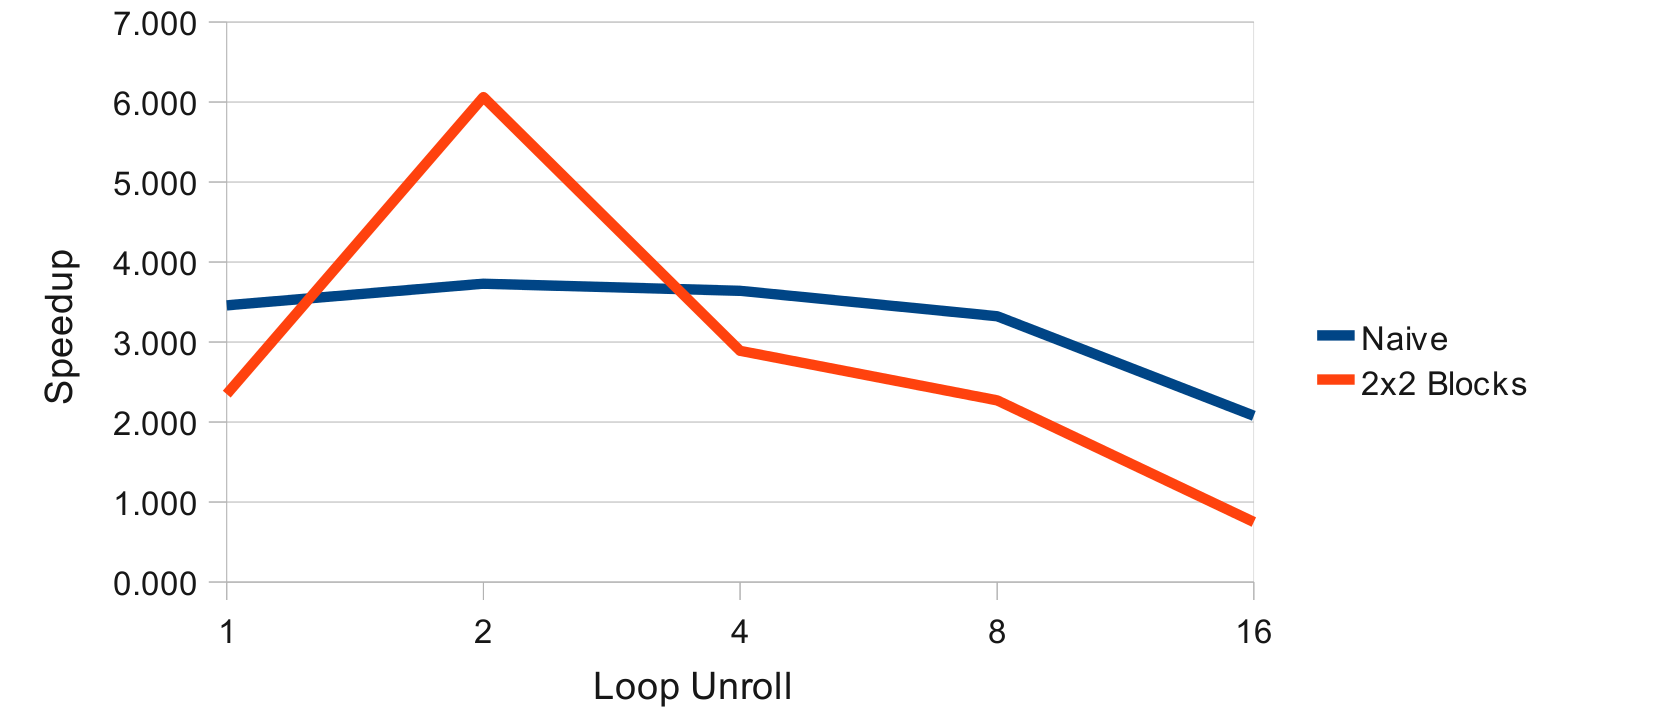
\includegraphics[clip]{unrolling}
\end{center}
\caption{Performance of 4k Matrix Multiplication with Unrolled Loops}\label{unroll}
\end{figure}

\section{Conclusion}
Hai \cite{Berlin:1990}.

\bibliography{bacon}{}
\bibliographystyle{splncs03}
\end{document}
